\documentclass[12pt]{beamer}

%%%%%%%%%%%%
% Packages %
%%%%%%%%%%%%

\usepackage[english]{babel}
\usepackage{sleek}
\usepackage{tikz}

%%%%%%%%%%%%%%%%
% Bibliography %
%%%%%%%%%%%%%%%%

\addbibresource{references.bib}

%%%%%%%%%%%%%%
% Title-page %
%%%%%%%%%%%%%%

\title{Arbitrary Marginal Neural Ratio Estimation for Simulation-based Inference}
\author{François Rozet, Antoine Wehenkel and Gilles Louppe}
\arxiv{2110.00449}
\github{francois-rozet/amnre}
\link{https://arxiv.org/abs/2110.00449}

%%%%%%%%%%%%
% Document %
%%%%%%%%%%%%

\begin{document}
\begin{frame}[t]
\begin{multicols}{2}

\section{A section title}

Some section contents, followed by a diagram, followed by a dummy paragraph.

\begin{figure}
    \vspace{0.5\baselineskip}
    \centering
    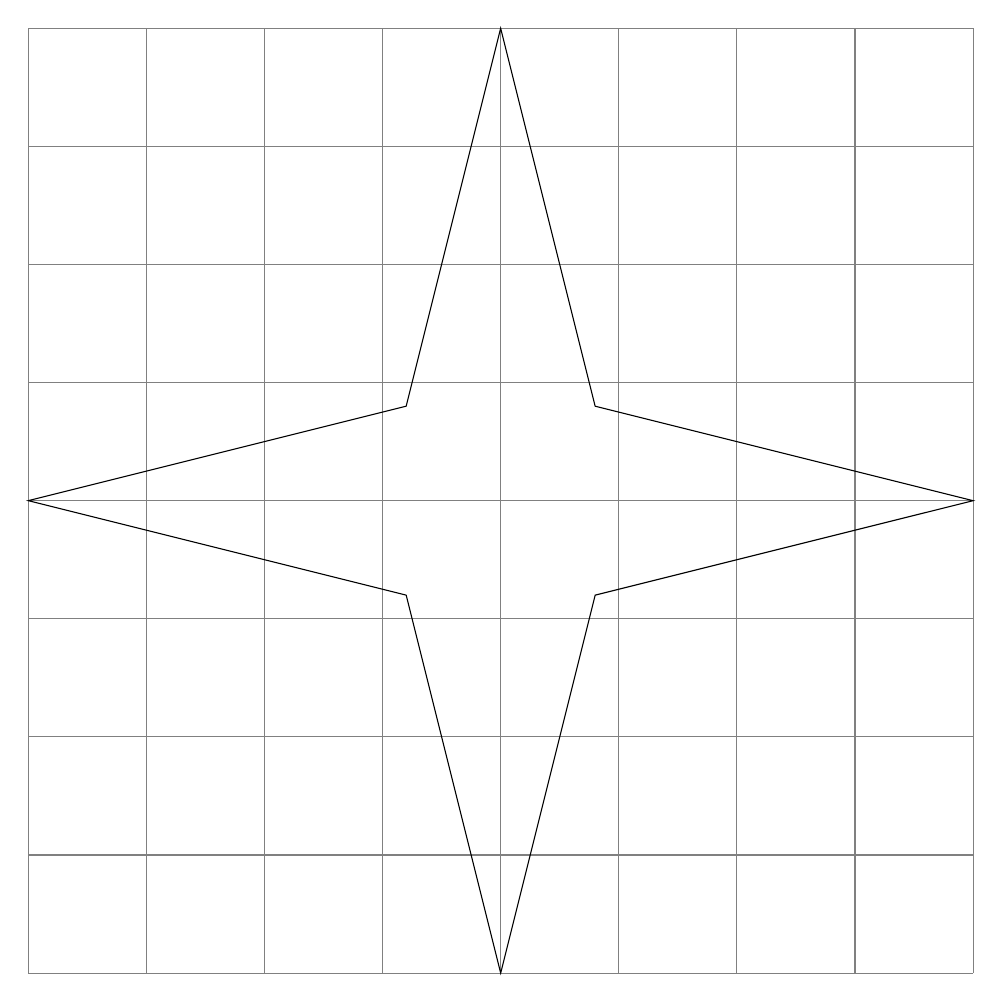
\begin{tikzpicture}[scale=6]
        \draw[step=0.25cm,color=gray] (-1,-1) grid (1,1);
        \draw (1,0) -- (0.2,0.2) -- (0,1) -- (-0.2,0.2) -- (-1,0)
            -- (-0.2,-0.2) -- (0,-1) -- (0.2,-0.2) -- cycle;
    \end{tikzpicture}
    \caption{A figure caption.}
\end{figure}

Lorem ipsum dolor sit amet, consectetur adipiscing elit. Morbi ultricies eget libero ac ullamcorper. Integer et euismod ante. Aenean vestibulum lobortis augue, ut lobortis turpis rhoncus sed. Proin feugiat nibh a lacinia dignissim. Proin scelerisque, risus eget tempor fermentum, \alert{ex turpis condimentum urna}, quis malesuada sapien arcu eu purus.

\section{A section containing a list}

Curabitur eu libero vehicula, cursus est fringilla, luctus est. Morbi consectetur mauris quam, at finibus elit auctor ac. Aliquam erat volutpat. Aenean at nisl ut ex ullamcorper eleifend et eu augue. Aenean quis velit tristique odio convallis ultrices a ac odio.

\begin{itemize}
    \item \textbf{Fusce dapibus tellus} vel tellus semper finibus. In consequat, nibh sed mattis luctus, augue diam fermentum lectus.
    \item \textbf{In euismod erat metus} non ex. Vestibulum luctus augue in mi condimentum, at sollicitudin lorem viverra.
    \item \textbf{Suspendisse vulputate} mauris vel placerat consectetur. Mauris semper, purus ac hendrerit molestie, elit mi dignissim odio, in suscipit felis sapien vel ex.
\end{itemize}

Aenean tincidunt risus eros, at gravida lorem sagittis vel. Vestibulum ante ipsum primis in faucibus orci luctus et ultrices posuere cubilia Curae.

\section{A section containing an enumerated list}

Vivamus congue volutpat elit non semper. Praesent molestie nec erat ac interdum. In quis suscipit erat. \alert{\textbf{Phasellus mauris felis}}, molestie ac pharetra quis, tempus nec ante. Donec finibus ante vel purus mollis fermentum.

\begin{enumerate}
    \item \textbf{Morbi mauris purus}, egestas at vehicula et, convallis accumsan orci. Orci varius natoque penatibus et magnis dis parturient montes, nascetur ridiculus mus.
    \item \textbf{Cras vehicula blandit urna ut maximus}. Aliquam blandit nec massa ac sollicitudin. Curabitur cursus, metus nec imperdiet bibendum, velit lectus faucibus dolor, quis gravida metus mauris gravida turpis.
    \item \textbf{Vestibulum et massa diam}. Phasellus fermentum augue non nulla accumsan, non rhoncus lectus condimentum.
\end{enumerate}

\section{A section containing some math}

Nullam non est elit. In eu ornare justo. Maecenas porttitor sodales lacus, ut cursus augue sodales ac.
$$
    \int_{-\infty}^{\infty} e^{-x^2}\,dx = \sqrt{\pi}
$$
Interdum et malesuada fames $\{1, 4, 9, \ldots\}$ ac ante ipsum primis in faucibus. Cras eleifend dolor eu nulla suscipit suscipit. Sed lobortis non felis id vulputate.

Praesent consectetur mi $x^2 + y^2$ metus, nec vestibulum justo viverra nec. Proin eget nulla pretium, egestas magna aliquam, mollis neque. Vivamus dictum $\bm{u}^\intercal\bm{v}$ sagittis odio, vel porta erat congue sed. Maecenas ut dolor quis arcu auctor porttitor.

\columnbreak

\section{Nullam vel erat at velit convallis laoreet}

Class aptent taciti sociosqu ad litora torquent per conubia nostra, per inceptos himenaeos. Phasellus libero enim, gravida sed erat sit amet, scelerisque congue diam. Fusce dapibus dui ut augue pulvinar iaculis.

\begin{table}
    \vspace{0.5\baselineskip}
    \centering
    \begin{tabular}{lrrc}
        \toprule
        \textbf{First} & \textbf{Second} & \textbf{Third} & \textbf{Fourth} \\
        \midrule
        Foo & 13.37 & 384,394 & $\alpha$ \\
        Bar & 2.17 & 1,392 & $\beta$ \\
        Baz & 3.14 & 83,742 & $\delta$ \\
        Qux & 7.59 & 974 & $\gamma$ \\
        \bottomrule
    \end{tabular}
    \caption{A table caption.}
\end{table}

Donec quis posuere ligula. Nunc feugiat elit a mi malesuada consequat. Sed imperdiet augue ac nibh aliquet tristique. Aenean eu tortor vulputate, eleifend lorem in, dictum urna. Proin auctor ante in augue tincidunt tempor. Proin pellentesque vulputate odio, ac gravida nulla posuere efficitur. Aenean at velit vel dolor blandit molestie. Mauris laoreet commodo quam, non luctus nibh ullamcorper in. Class aptent taciti sociosqu ad litora torquent per conubia nostra, per inceptos himenaeos.

\vspace{0.25\baselineskip}

\begin{block}{Dogec tempus}
    Vivamus vitae maximus nibh. Fusce gravida bibendum nisi, ut scelerisque quam pellentesque vitae. Nunc feugiat, magna ac lobortis venenatis, tellus lorem blandit massa, sed rhoncus est mi nec libero. Suspendisse potenti. Etiam pulvinar dignissim rhoncus. Ut et fermentum sapien. Nunc quis ante nec felis imperdiet iaculis. Aliquam ultricies, \alert{felis porta eleifend} pellentesque, nulla leo molestie ipsum, et iaculis tellus erat ut est.
\end{block}

\vspace{0.25\baselineskip}

\begin{alertblock}{Quisque aliquam tellus}
    Suspendisse at orci feugiat, pharetra mauris vel, placerat turpis. Nulla sit amet porttitor dolor. Curabitur auctor augue eu nisl rhoncus congue. Donec ligula mi, hendrerit vitae metus eget, sodales lobortis lacus. Cras libero velit, mollis eu ultricies nec, porttitor non nunc. Quisque turpis elit, blandit ut tincidunt ac, faucibus non nisl. Donec dictum imperdiet lorem, eu elementum mauris volutpat dignissim.
\end{alertblock}

\section{References}

\nocite{einstein}
\nocite{knuthwebsite}
\nocite{dirac}
\printbibliography[heading=none]

\end{multicols}
\end{frame}
\end{document}
